\documentclass[12pt,a4paper]{article}
\usepackage[utf8]{inputenc}
\usepackage{amsmath}
\usepackage{breqn}
\usepackage{amsfonts}
\usepackage{amssymb}
\usepackage{graphicx}
\usepackage[margin=0.8in]{geometry}


\begin{document}
\title{\vspace{70mm}\Huge Experimento 01 - Pêndulo Composto}
\author{ Giovani Garuffi\qquad\hfill
		\textit {RA: 155559}\protect\\
		João Baraldi\hfill
		\textit{RA: 158044}\protect\\
		Lauro Cruz\hfill
		\textit{RA: 156175}\protect\\
		Lucas Schanner\hfill
		\textit{RA: 156412}\protect\\
		Pedro Stringhini\hfill
		\textit {RA: 156983}								
		}
\maketitle
\newpage
\section{Resumo}

O experimento é um estudo do pêndulo composto (formado por uma barra de alumínio e outra de ferro acoplada) e seu comportamento. Medidas as massas das barras, é realizada a cronometragem dos períodos de oscilação do pêndulo para diferentes configurações.\\ %Bem, eu prefiro sem salto de linha (há controvérsias).
São registrados valores dos períodos (T) relacionados às diferentes distâncias entre eixo de rotação e centro de massa (D) do pêndulo, variantes conforme a configração. Depois, é feito o gráfico $T^2D$ x $D^2$, representando a função afim $T^2D = (4pi^2/g)D^2 + 4pi^2k^2/g$ e sendo k o raio de giração do pêndulo. Assim, utilizando o método dos mínimos quadrados, foram obtidos os valores do raio de giração $k = (0.465 \pm 0.001)m$ e da aceleração da gravidade $g = (10.34 \pm 0.06) m/s^2$. Tal valor não consta dentro do esperado, considerando que  teoricamente $g\approx9.8 m/s^2$, o que não foi abrangido pela margem de erro. Como o momento de inércia do pêndulo em relação ao centro de massa é dado pela fórmula $(M_1 + M_2)*k^2$, foi possível calcular seu valor como $Icm = (0.28 \pm 0.02)Kg.m^2$.
\section{Objetivos}
Investigar o movimento de um pêndulo e seu comportamento relacionando as grandezas sobre ele atuantes, como centro de massa, raio de giração e momento de inércia.

\section{Procedimento Experimental e Coleta de Dados}
\subsection{Procedimento}

Um pêndulo foi montado com uma barra metálica maior de alumínio e outra adicional de ferro colocada em sua extremidade inferior. Depois de devidamente medido (com fita métrica) e pesado (com balança analítica), ele foi fixado em um eixo de suspensão. No ponto mais baixo da trajetória do instrumento, foi acoplado um photogate ligado a um cronômetro inteligente adaptado a medição dos periodos (T) de oscilação do pêndulo. Assim, com o devido cuidado de acionar uma oscilação de ângulo menor que 15 graus para efeitos de aproximação, foram medidos tais períodos 7 vezes em cada uma das 6 configurações escolhidas, diferenciadas pela distância entre o eixo fixo e o centro de massa do pêndulo. As medições foram anotadas e estão inclusas em sua totalidade no relatório. A montagem do experimento pode ser vista nas imagens a seguir.\\

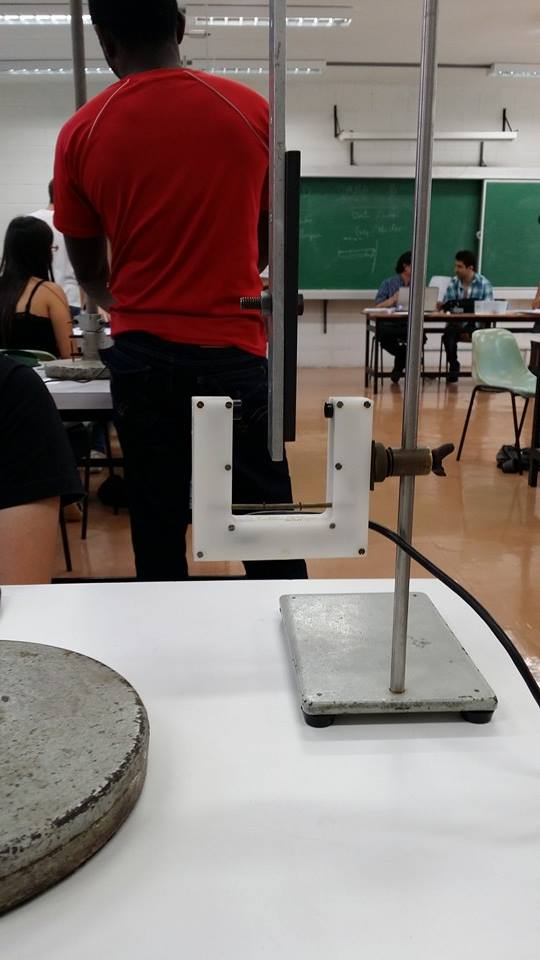
\includegraphics[scale=0.30]{1.jpg} 
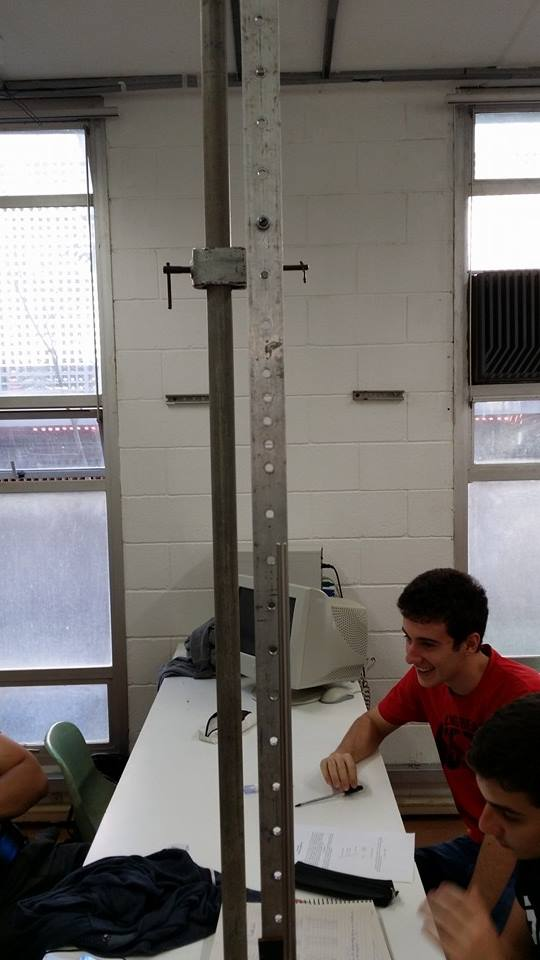
\includegraphics[scale=0.30]{2.jpg} 
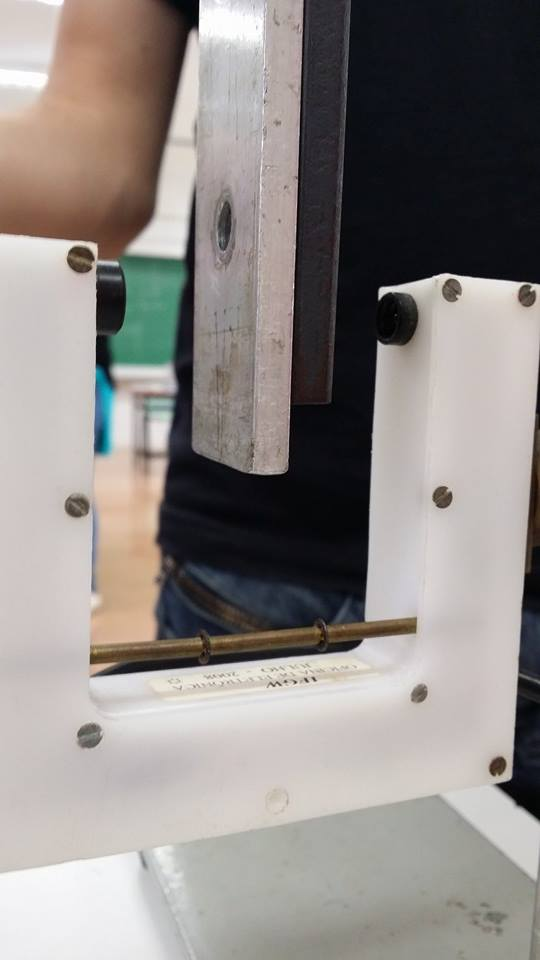
\includegraphics[scale=0.30]{3.jpg} 
\emph{Figuras 1, 2 e 3: Montagem do experimento.}




\subsection{Dados Obtidos}

As medidas da posição do centro de massa da barra maior de alumínio $(x_1)$ e da menor de ferro $(x_2)$, aproximando-as como corpos homogêneos e fixando a origem na extremidade inferior do pêndulo, são equivalentes à metade do comprimento delas, resultando em: \\
$$ x_1 = (0.0915 \pm 0.0005) M$$
$$ x_2 = (0.7420 \pm 0.0005) M$$
E suas respectivas Massas:\\
$$ M_1 = (347.3 \pm 0.1) g $$
$$ M_2 = (929.5 \pm 0.1) g $$


As medidas de periodo tomadas estão presentes na seguinte tabela, relacionadas às distâncias do eixo de rotação à extremidade inferior do pêndulo. \\

\begin{table}[!htbp]
\centering
\textbf {Tabela 1: Medidas do Periodo de oscilação do pêndulo e suas médias aritméticas relacionadas à distância X do eixo de rotação à extremidade inferior do pêndulo}\\ 	%% Preferi reduzir o título e colocar os erros (mesmo os ctes) na tabela. Podemos mudar isso de novo caso queira.

\def\arraystretch{1.5}
\begin{tabular}{|l| c c c c c c c|r|}
\hline 
X (metro) & \multicolumn{7}{c|}{Períodos (s)} & {Valor Médio (s)} \\ 
\hline
$1.0450\pm0.0005$ & 1.8866 & 1.8878 & 1.8881 & 1.8869 & 1.8867 & 1.8862 & 1.8864 & $1.8870 \pm 0.0003 $ \\
\hline
$0.9900\pm0.0005$ & 1.8877 & 1.8882 & 1.888 & 1.888 & 1.8851 & 1.8874 & 1.8869 & $1.8873 \pm 0.0004 $\\
\hline
$0.9400\pm0.0005$ & 1.9018 & 1.9026 & 1.9020 & 1.9048 & 1.902 & 1.9016 & 1.8985 & $1.9019 \pm 0.0007$\\
\hline
$0.8900\pm0.0005$ & 1.9341 & 1.9349 & 1.9345 & 1.9342 & 1.9335 & 1.9335 & 1.9340 & $1.9341 \pm 0.0002$\\
\hline
$0.8400\pm0.0005$ & 1.9956 & 1.9957 & 1.9947 & 1.9947 & 1.9946 & 1.9986 & 1.9935 & $1.9953 \pm 0.0006$\\
\hline
$0.7915\pm0.0005$ & 2.1042 & 2.1027 & 2.1027 & 2.1024 & 2.1026 & 2.1023 & 2.1019 & $2.1027 \pm 0.0003 $\\
\hline
\end{tabular}

\emph{Nota: erro instrumental do cronômetro = $0.0001$s.\\ erro total calculado com base nos erros estatísticos e instrumentais.}
\end{table}
\newpage


\section{Análise dos Resultados e Discussões}
\subsection{Centro de Massa}
A posição do do centro de Massa relativo à extremidade inferior pode ser calculado como\\
$$ x_{cm} = \frac{x_1 \cdot M_1 + x_2 \cdot M_2}{M_1 + M_2} = 0.5552 m $$\\ \\
O erro associado a essa medida, propagado a partir dos erros de $x_1$, $M_1$, $x_2$ e $M_2$ é de 


% PUTA QUE O PARIU

$$\sqrt{\Delta m_{1}^{2} \left(\frac{x_{1}}{m_{1} + m_{2}} - \frac{m_{1} x_{1} + m_{2} x_{2}}{\left(m_{1} +  m_{2}\right)^{2}}\right)^{2} + \Delta m_{2}^{2} \left(\frac{x_{2}}{m_{1} + m_{2}} - \frac{m_{1} x_{1} + m_{2} x_{2}}{\left(m_{1} + m_{2}\right)^{2}}\right)^{2} + \frac{\Delta x_{1}^{2} m_{1}^{2}}{\left(m_{1} + m_{2}\right)^{2}} + \frac{\Delta x_{2}^{2} m_{2}^{2}}{\left(m_{1} + m_{2}\right)^{2}}} $$
$$ = \pm 0.0003m $$


\subsection{Períodos}
O período de oscilação do pêndulo, T, para pequenos ângulos de oscilação, é dado por
$$ T = 2 \pi \sqrt{\frac{I_0}{Mgd}} $$
Onde $I_0$ é o momento de inércia do pendulo em relação ao ponto de suspensão.
Utilizando o teorema dos eixos paralelos, e lembrando que $I_{cm} = Mk^2$, sendo 
$k$ o raio de giração, deduz-se a equação
$$ T = 2\pi\sqrt{\frac{D + \frac{k^2}{D}}{g}} $$ 
que pode ser reescrita como 
\begin{equation} \label{eq:funcao}
 T^2D = \frac{4\pi^2}{g} \cdot D^2 + \frac{4\pi^2}{g} \cdot k^2 
\end{equation}
Sendo que $$D = X - x_{cm} $$ 
$$ \Delta D = \sqrt{{\Delta X}^2 + {\Delta x_{cm}}^2}  = 0.0003 m$$
Percebe-se que deve existir uma relação linear entre $T^2D$ e $D^2$.






\begin{table}[!htbp]
\centering
\def\arraystretch{1.5}

\textbf {Tabela 2: Periodos de oscilação relativos à distância $D$ do eixo de rotação ao centro de massa do pêndulo}\\
\begin{tabular}{|c|c|c|c|}
\hline
D (M)& T(s) & $D^2$ & $T^2D$ \\
\hline
$0.4897\pm0.0003$ & $1.8870 \pm 0.0003$ & $0.2398\pm0.0003$ & $1.744 \pm 0.001$\\
\hline
$0.4347\pm0.0003$ & $1.8873 \pm 0.0004$ & $0.1890\pm0.0003$ & $1.549 \pm 0.001$\\
\hline
$0.3847\pm0.0003$ & $1.9019 \pm 0.0007$ & $0.1480\pm0.0002$ & $1.392 \pm 0.001$\\
\hline
$0.3347\pm0.0003$ & $1.9341 \pm 0.0002$ & $0.1120\pm0.0002$ & $1.252 \pm 0.001$\\
\hline
$0.2847\pm0.0003$ & $1.9953 \pm 0.0006$ & $0.0810\pm0.0002$ & $1.134 \pm 0.001$\\
\hline
$0.2362\pm0.0003$ & $2.1027 \pm 0.0003$ & $0.0558\pm0.0001$ & $1.045 \pm 0.001$\\
\hline
\end{tabular}
\\
\emph {Nota: Erro em D propagado a partir do erro em X e em $x_{cm}$.\\
			Erro em $T^2D$ foi propagado a partir do erro em D e em T.\\}
\end{table}



Fazendo a regressão linear de $T^2D$ X $D^2$ por mínimos quadrados, obtem-se os coeficientes 
$$ a = 3.82 \pm 0.02 $$ 
 $$ b = 0.827 \pm 0.003 $$
onde $a$ é o coeficiente angular e $b$ é o coeficiente linear. A reta formada pode ser vista no Gráfico 1, sobreposta aos pontos da tabela.

\begin{figure}[!hbtbp]

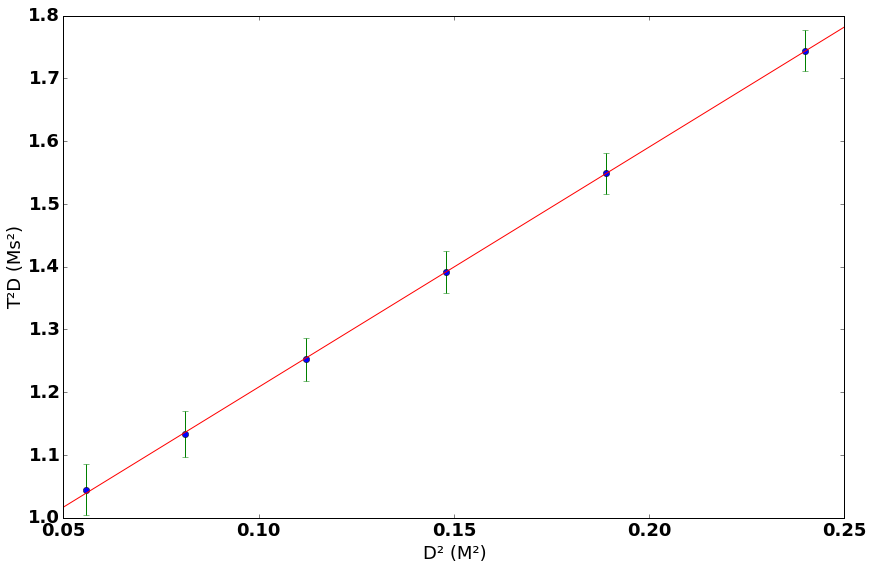
\includegraphics[scale=0.55]{index.png} 
\emph{Figura 4: Gráfico 1: $T^2D$ em função de $D^2$. Nota-se que os dados coletados se encaixam muito bem em uma projeção linear.}

\label{fig:Grafico}
\end{figure}
\subsection{Gravidade}
A interpretação física do coeficiente angular encontrado é, por (\ref{eq:funcao}),
 $$ a = \frac{4\pi^2}{g} = 3.82 \pm 0.02$$
  logo podemos encontrar $g$ como 

  $$ g = \frac{4\pi^2}{3.82} = 10.34 m/s^2 $$ 
  e seu erro associado, propagado a partir do erro em $a$ é
  $$ \Delta g = \frac{4\pi^2}{a^2} \cdot \Delta a = \pm 0.06 m/s^2 $$
  O valor da gravidade calculado não está de acordo com o valor conhecido de $g \approx 9.8m/s^2$.

\subsection{Raio de giração}

A interpretação física do coeficiente linear, a partir de (\ref{eq:funcao}), é 
$$ b = \frac{4\pi^2}{g} \cdot k^2 = 0.827 \pm 0.003 $$
logo, o raio de giração pode ser obtido por:
$$ k = \sqrt{\frac{g \cdot b}{4\pi^2}} = 0.465 m $$
E seu erro, calculado por:
$$ \Delta k =
\sqrt{\frac{\Delta b^{2} g}{16 \pi^{2} b} + \frac{\Delta g^{2} b}{16 \pi^{2} g}} 
 =  \pm 0.002  m$$

\subsection{Momento de Inércia}
O momento de inércia pode ser descrito em função do raio de giração como 
$$ I_{cm}  = (m_1 + m_2)k^2 $$
Substituindo os valores, obtemos:
$$ I_{cm}  = 0.282 (m^2 \cdot Kg)$$
E o erro $ \Delta I_{cm}$ pode ser calculado a partir da expressão 
$$\Delta I_{cm}  =\sqrt{(2mk \cdot \Delta k)^2 + (k^2 \cdot \Delta M)^2} = \pm 0.006 (m \cdot Kg) $$

\section{Conclusões}
Como o experimento falhou em encontrar um valor para a gravidade de acordo com a teoria conhecida atualmente, também não há grande confiabilidade nos valores encontrados do Raio de Giração (K) e Momento de Inercia (I), considerando as imprecisões apresentadas.

% Stringhini dê seu show
Esse erro pode ser explicado, ainda que parcialmente pelo erro da aproximação $tg(\theta) = sen(\theta) = \theta$, utilizada para se obter a igualdade $ T = 2\pi\sqrt{\frac{D + \frac{k^2}{D}}{g}} $. Buscando maior precisão, o ideal estaria em desconsiderar tal aproximação e utilizar a versão extensa da relação. No entanto, tal versão, supondo uma angulação $\theta = 20\,^{\circ}$, corrigiria cerca de $1\%$ do erro, o que não é suficiente em si. Outras fontes de erro são as possíveis imprecisões instrumentais de alguma forma desconsideradas, incluindo o conhecimento apenas superficial do modo "pêndulo" apresentado no photogate/cronômetro inteligente.

Novos estudos precisam ser feitos, de modo que se utilize modelagem mais precisa para obter resultados melhores.

\end{document}
